\usetikzlibrary{arrows.meta,calc,positioning}
\begin{figure}[htbp]
  \centering
  \makebox[\textwidth][c]{%
  \resizebox{0.98\textwidth}{!}{%
  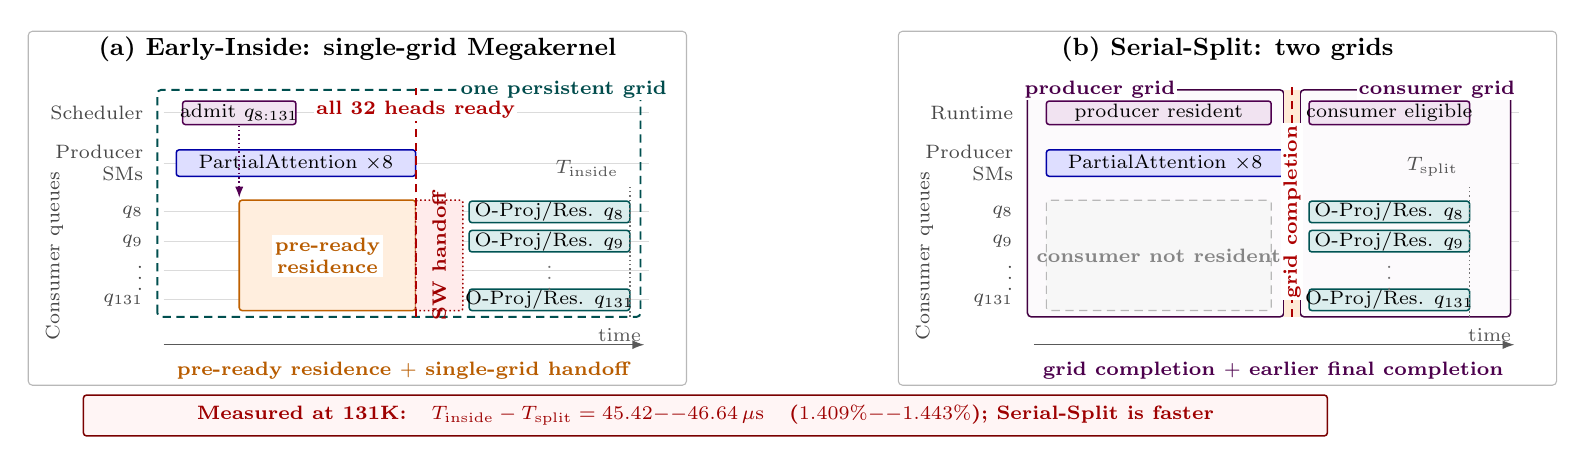
\begin{tikzpicture}[
      x=0.80cm,
      y=0.62cm,
      font=\sffamily\footnotesize,
      panel/.style={draw=black!28, rounded corners=1.5pt,
                    line width=0.4pt},
      lane/.style={draw=black!14, line width=0.3pt},
      lanelabel/.style={anchor=east, font=\scriptsize, text=black!72},
      producer/.style={draw=blue!65!black, fill=blue!13,
                       rounded corners=1pt, line width=0.55pt},
      consumer/.style={draw=teal!65!black, fill=teal!14,
                       rounded corners=1pt, line width=0.55pt},
      scheduler/.style={draw=violet!62!black, fill=violet!11,
                        rounded corners=1pt, line width=0.55pt},
      preready/.style={draw=orange!75!black, fill=orange!13,
                       rounded corners=1pt, line width=0.55pt},
      handoff/.style={draw=red!62!black, fill=red!8,
                      densely dotted, rounded corners=0.8pt,
                      line width=0.55pt},
      inactive/.style={draw=black!28, fill=black!3, densely dashed,
                       rounded corners=1pt, line width=0.4pt},
      persistgrid/.style={draw=teal!62!black, densely dashed,
                          rounded corners=1.4pt, line width=0.7pt},
      physicalgrid/.style={draw=violet!52!black, fill=violet!2,
                           rounded corners=1.4pt, line width=0.55pt},
      readyline/.style={draw=red!68!black, densely dashed,
                        line width=0.65pt},
      finishline/.style={draw=black!55, densely dotted,
                         line width=0.55pt},
      flow/.style={-{Latex[length=1.4mm]}, line width=0.55pt},
      result/.style={draw=red!48!black, fill=red!4,
                     rounded corners=1.2pt, line width=0.55pt}
    ]

    % ====================================================================
    % (a) Early-Inside
    % ====================================================================
    \begin{scope}[xshift=0cm]
      \draw[panel] (0,0) rectangle (10.45,7.25);
      \node[font=\small\bfseries] at (5.225,6.88)
        {(a) Early-Inside: single-grid Megakernel};

      % Shared resource lanes.
      \foreach \yy in {5.58,4.55,3.55,2.95,2.35,1.75} {
        \draw[lane] (2.15,\yy) -- (9.85,\yy);
      }
      \node[lanelabel] at (1.98,5.58) {Scheduler};
      \node[lanelabel,align=right] at (1.98,4.55) {Producer\\SMs};
      \node[font=\scriptsize,rotate=90,text=black!72] at (0.42,2.65)
        {Consumer queues};
      \node[lanelabel] at (1.98,3.55) {$q_8$};
      \node[lanelabel] at (1.98,2.95) {$q_9$};
      \node[lanelabel] at (1.98,2.35) {$\vdots$};
      \node[lanelabel] at (1.98,1.75) {$q_{131}$};

      % One persistent grid contains scheduler, producer, and consumers.
      \draw[persistgrid] (2.05,1.40) rectangle (9.72,6.05);
      \node[font=\scriptsize\bfseries,fill=white,inner sep=0.7pt,
            text=teal!60!black] at (8.50,6.05)
        {one persistent grid};

      % Device-side early admission.
      \draw[scheduler] (2.45,5.34) rectangle (4.25,5.82);
      \node[font=\scriptsize] at (3.35,5.58)
        {admit $q_{8{:}131}$};

      % Producer stage: eight tasks collectively make 32 query heads ready.
      \draw[producer] (2.35,4.28) rectangle (6.15,4.82);
      \node[font=\scriptsize] at (4.25,4.55)
        {PartialAttention $\times 8$};

      % Consumers are resident before the shared full-ready condition.
      \draw[preready] (3.35,1.53) rectangle (6.15,3.79);
      \node[font=\scriptsize\bfseries,align=center,
            fill=white,inner sep=1.1pt,text=orange!72!black]
        at (4.75,2.65) {pre-ready\\residence};

      % After full readiness, the single-grid path still performs a software
      % task handoff before the main consumer body can run.  The measured result
      % below, rather than an individual micro-event, establishes the gap.
      \draw[handoff] (6.15,1.53) rectangle (6.90,3.79);
      \node[font=\scriptsize\bfseries,rotate=90,text=red!62!black]
        at (6.525,2.65) {SW handoff};

      % Global all-ready condition shared by every consumer.
      \draw[readyline] (6.15,1.40) -- (6.15,6.08);
      \node[font=\scriptsize\bfseries,fill=white,inner sep=0.8pt,
            text=red!68!black] at (6.15,5.64)
        {all 32 heads ready};

      % Main consumer computation can start only after full readiness.
      \foreach \yy/\qq in {3.55/8,2.95/9,1.75/131} {
        \draw[consumer] (7.00,\yy-0.22) rectangle (9.55,\yy+0.22);
        \node[font=\scriptsize] at (8.275,\yy)
          {O-Proj/Res. $q_{\qq}$};
      }
      \node[font=\scriptsize,text=black!55] at (8.275,2.35) {$\vdots$};

      % End-to-end completion marker on the shared schematic time scale.
      \draw[finishline] (9.55,1.40) -- (9.55,4.06);
      \node[font=\scriptsize\bfseries,anchor=south east,
            text=black!68] at (9.52,4.08) {$T_{\mathrm{inside}}$};

      % Admission marker links the scheduler decision to consumer residence.
      \draw[flow,draw=violet!65!black,densely dotted]
        (3.35,5.32) -- (3.35,3.84);

      \draw[-{Latex[length=1.5mm]},black!65]
        (2.15,0.83) -- (9.78,0.83)
        node[above left,inner sep=1pt,font=\scriptsize] {time};
      \node[font=\scriptsize\bfseries,text=orange!72!black]
        at (5.95,0.30)
        {pre-ready residence $+$ single-grid handoff};
    \end{scope}

    % ====================================================================
    % (b) Serial-Split
    % ====================================================================
    \begin{scope}[xshift=11.05cm]
      \draw[panel] (0,0) rectangle (10.45,7.25);
      \node[font=\small\bfseries] at (5.225,6.88)
        {(b) Serial-Split: two grids};

      % Identical resource lanes and horizontal time scale.
      \foreach \yy in {5.58,4.55,3.55,2.95,2.35,1.75} {
        \draw[lane] (2.15,\yy) -- (9.85,\yy);
      }
      \node[lanelabel] at (1.98,5.58) {Runtime};
      \node[lanelabel,align=right] at (1.98,4.55) {Producer\\SMs};
      \node[font=\scriptsize,rotate=90,text=black!72] at (0.42,2.65)
        {Consumer queues};
      \node[lanelabel] at (1.98,3.55) {$q_8$};
      \node[lanelabel] at (1.98,2.95) {$q_9$};
      \node[lanelabel] at (1.98,2.35) {$\vdots$};
      \node[lanelabel] at (1.98,1.75) {$q_{131}$};

      % Two physical grids separated at the full-ready cut.
      \draw[physicalgrid] (2.05,1.40) rectangle (6.12,6.05);
      \draw[physicalgrid] (6.38,1.40) rectangle (9.72,6.05);
      \node[font=\scriptsize\bfseries,fill=white,inner sep=0.7pt,
            text=violet!58!black] at (3.20,6.05) {producer grid};
      \node[font=\scriptsize\bfseries,fill=white,inner sep=0.7pt,
            text=violet!58!black] at (8.55,6.05) {consumer grid};

      \draw[scheduler] (2.35,5.34) rectangle (5.92,5.82);
      \node[font=\scriptsize] at (4.135,5.58)
        {producer resident};

      \draw[producer] (2.35,4.28) rectangle (6.12,4.82);
      \node[font=\scriptsize] at (4.235,4.55)
        {PartialAttention $\times 8$};

      % Consumer queues are not admitted while the producer grid is active.
      \draw[inactive] (2.35,1.53) rectangle (5.92,3.79);
      \node[font=\scriptsize\bfseries,align=center,text=black!48]
        at (4.135,2.65) {consumer not resident};

      % Physical completion expresses the shared all-ready condition.
      \fill[orange!16] (6.12,1.40) rectangle (6.38,6.05);
      \draw[readyline] (6.25,1.40) -- (6.25,6.10);
      \node[font=\scriptsize\bfseries,rotate=90,fill=white,inner sep=0.8pt,
            text=red!68!black] at (6.25,3.55)
        {grid completion};

      \draw[scheduler] (6.52,5.34) rectangle (9.07,5.82);
      \node[font=\scriptsize] at (7.795,5.58)
        {consumer eligible};

      % The same consumer code begins only after the physical boundary.
      \foreach \yy/\qq in {3.55/8,2.95/9,1.75/131} {
        \draw[consumer] (6.52,\yy-0.22) rectangle (9.07,\yy+0.22);
        \node[font=\scriptsize] at (7.795,\yy)
          {O-Proj/Res. $q_{\qq}$};
      }
      \node[font=\scriptsize,text=black!55] at (7.795,2.35) {$\vdots$};

      \draw[finishline] (9.07,1.40) -- (9.07,4.06);
      \node[font=\scriptsize\bfseries,anchor=south east,
            text=black!68] at (9.04,4.08) {$T_{\mathrm{split}}$};

      \draw[-{Latex[length=1.5mm]},black!65]
        (2.15,0.83) -- (9.78,0.83)
        node[above left,inner sep=1pt,font=\scriptsize] {time};
      \node[font=\scriptsize\bfseries,text=violet!60!black]
        at (5.95,0.30)
        {grid completion $+$ earlier final completion};
    \end{scope}

    % The measured result makes the performance direction explicit.  The
    % timeline above is schematic; the numeric difference is the experiment.
    \node[result,minimum width=15.8cm,minimum height=0.52cm,
          font=\scriptsize\bfseries,text=red!62!black] at (10.75,-0.62)
      {Measured at 131K:\quad
       $T_{\mathrm{inside}}-T_{\mathrm{split}}
         =45.42\text{--}46.64\,\mu\mathrm{s}$\quad
       ($1.409\%\text{--}1.443\%$); Serial-Split is faster};

  \end{tikzpicture}%
  }}%
  \caption{Hazy \texttt{PartialAttention}$\rightarrow$\texttt{O\_ProjResidual} 的 SM--时间执行结构。Early-Inside 中，queues 8--131 在 32 个 query heads 全量就绪前进入 consumer 路径，形成 pre-ready residence interval；Serial-Split 由 producer grid completion 统一放行 consumer grid。两种方案保持 task code、queue mapping、task/noop slots 和 instruction bytes 一致。橙色区间对应后续 admission-gated 对照与设备端时间戳所分解的关键阶段。}
  \label{fig:hazy-boundary}
\end{figure}
